\documentclass[oneside,numbers]{ezthesis}
%% # Opciones disponibles para el documento #
%%
%% Las opciones con un (*) son las opciones predeterminadas.
%%
%% Modo de compilar:
%%   draft            - borrador con marcas de fecha y sin im'agenes
%%   draftmarks       - borrador con marcas de fecha y con im'agenes
%%   final (*)        - version final de la tesis
%%
%% Tama'no de papel:
%%   letterpaper (*)  - tama'no carta (Am'erica)
%%   a4paper          - tama'no A4    (Europa)
%%
%% Formato de impresi'on:
%%   oneside          - hojas impresas por un solo lado
%%   twoside (*)      - hijas impresas por ambos lados
%%
%% Tama'no de letra:
%%   10pt, 11pt, o 12pt (*)
%%
%% Espaciado entre renglones:
%%   singlespace      - espacio sencillo
%%   onehalfspace (*) - espacio de 1.5
%%   doublespace      - a doble espacio
%%
%% Formato de las referencias bibliogr'aficas:
%%   numbers          - numeradas, p.e. [1]
%%   authoryear (*)   - por autor y a'no, p.e. (Newton, 1997)
%%
%% Opciones adicionales:
%%   spanish         - tesis escrita en espa'nol
%%
%% Desactivar opciones especiales:
%%   nobibtoc   - no incluir la bibiolgraf'ia en el 'Indice general
%%   nofancyhdr - no incluir "fancyhdr" para producir los encabezados
%%   nocolors   - no incluir "xcolor" para producir ligas con colores
%%   nographicx - no incluir "graphicx" para insertar gr'aficos
%%   nonatbib   - no incluir "natbib" para administrar la bibliograf'ia

%% Paquetes adicionales requeridos se pueden agregar tambi'en aqu'i.
%% Por ejemplo:
%\usepackage{subfig}
%\usepackage{multirow}
\usepackage{rotating,booktabs}
\usepackage{graphicx}
\usepackage{subfigure} % subfiguras
\graphicspath{{./img/}}
\DeclareGraphicsExtensions{.jpg,.png}
\usepackage{lscape}
\PassOptionsToPackage{USenglish}{babel}
\usepackage[USenglish]{babel} % espanol, ingles
\usepackage{multirow, array} %para mover el ancho de las tablas.
\renewcommand{\baselinestretch}{2}
\usepackage{vmargin}
\setcitestyle{numbers,super}

%\nocite{*}


\setpapersize{USletter}
\setmargins{3.2cm}       % margen izquierdo
{2.5cm}                        % margen superior
{15cm}                      % anchura del texto
{20cm}                    % altura del texto
{10pt}                           % altura de los encabezados
{1cm}                           % espacio entre el texto y los encabezados
{10pt}                             % altura del pie de página
{1cm}                           % espacio entre el texto y el pie de página

\usepackage{caption}
\usepackage{subfig}

\usepackage{amssymb, amsmath, amsbsy} % simbolitos
\usepackage{upgreek} % para poner letras griegas sin cursiva
\usepackage{cancel} % para tachar
\usepackage{mathdots} % para el comando \iddots
\usepackage{mathrsfs} % para formato de letra
\usepackage{stackrel} % para el comando \stackbin
\usepackage{enumerate} %para viñetas
%\usepackage{algpseudocode} %Para el apendice.
\usepackage{algorithm}
\usepackage{algorithmic}
\usepackage{listings}
\usepackage{rotating}
\usepackage{lscape}
%\usepackage{algpseudocode}
%\usepackage{pifont}
\usepackage{framed, color}
\usepackage[verbose]{placeins}
%\usepackage[ngerman]{babel}
\usepackage{blindtext}

\definecolor{shadecolor}{rgb}{1,0.8,0.3}




%% # Datos del documento #
%% Nota que los acentos se deben escribir: \'a, \'e, \'i, etc.
%% La letra n con tilde es: \~n.

%\author{Francisco Javier Arce C\'ardenas}
%\title{Tesis Doctoral}
%\degree{Doctor en Ciencias}
%\supervisor{Jos\'e Mario Garc\'ia Valdez}
%\institution{Instituto Tecnol\'ogico de Tijuana}
%\faculty{Ciencias de la computac\'ion}
%\department{Departamento de Sistemas Computacionales}

%% # M'argenes del documento #
%% 
%% Quitar el comentario en la siguiente linea para austar los m'argenes del
%% documento. Leer la documentaci'on de "geometry" para m'as informaci'on.

%\geometry{top=40mm,bottom=33mm,inner=40mm,outer=25mm}

%% El siguiente comando agrega ligas activas en el documento para las
%% referencias cruzadas y citas bibliogr'aficas. Tiene que ser *la 'ultima*
%% instrucci'on antes de \begin{document}.
\hyperlinking
\makeindex
\begin{document}
\pagenumbering{Roman}
%% En esta secci'on se describe la estructura del documento de la tesis.
%% Consulta los reglamentos de tu universidad para determinar el orden
%% y la cantidad de secciones que debes de incluir.

%% # Portada de la tesis #
%% Mirar el archivo "titlepage.tex" para los detalles.
%\include{titlepage}
%\include{knowledgements}
%\include{abstract}


%% # 'Indices y listas de contenido #
%% Quitar los comentarios en las lineas siguientes para obtener listas de
%% figuras y cuadros/tablas.
\tableofcontents
\listoffigures
\listoftables
%%\clearpage
%% # Capitulos #
%% Por cada cap'itulo hay que crear un nuevo archivo e incluirlo aqu'i.
%% Mirar el archivo "intro.tex" para un ejemplo y recomendaciones para
%% escribir.
\pagenumbering{arabic}
\setcounter{page}{1}
\chapter{Introduction} \label{introduction} 

The purpose of this research is to contribute in the diverse forms of use of the interactive learning environments by proposing a learning environment, we based the content management with an adaptive hypermedia approach and 
with the development of a new type of learning object to be adapted to the learning environment.
This environment use various devices that were capable of running a web browser, non-relational data bases for information exchange and some sensors like cameras and Kinect 2 were used. In addition we implemented a way to predict the level of user attention
which it was compared against information obtained by a video taken from the user doing the activity.

\section{Motivation}
There are many types of learning environments starting from the most basic that exist almost from the beginning of civilization where a person is able to learn based on their current context.
For example the first humans who needed to hunt them could take decisions and adapt to the situation and perform the task that was to hunt an animal to obtain food, in more recent times we can relate to the classrooms of schools, and currently including technology these Environments can be configurable and adapt to a particular context (the user).When a user uses learning environments the themes are usually flat and have the same content for everyone. In addition, users think and assimilate information in a different way which makes it more attractive to have a learning environment that adapts to the learning styles of the users and why not to the user preferences.

Nowadays most interactive museums work stations or exhibits like we see on the figure 1.1, where users come to the station to interact with or receive information by reversing some time on it until it passes to the next station, where the display will probably showed relevant information for the person but if this information is not shown to digestible way (processed so that it is attractive to the user) the user will probably spend less time or not time at all at the station. This expose the lack of adaptation of the exhibits in some interactive museums or standard museums. in order to ensure that the information and how is presented to the user is broadly engaging. 
\begin{figure}[ht!]  
\centering  
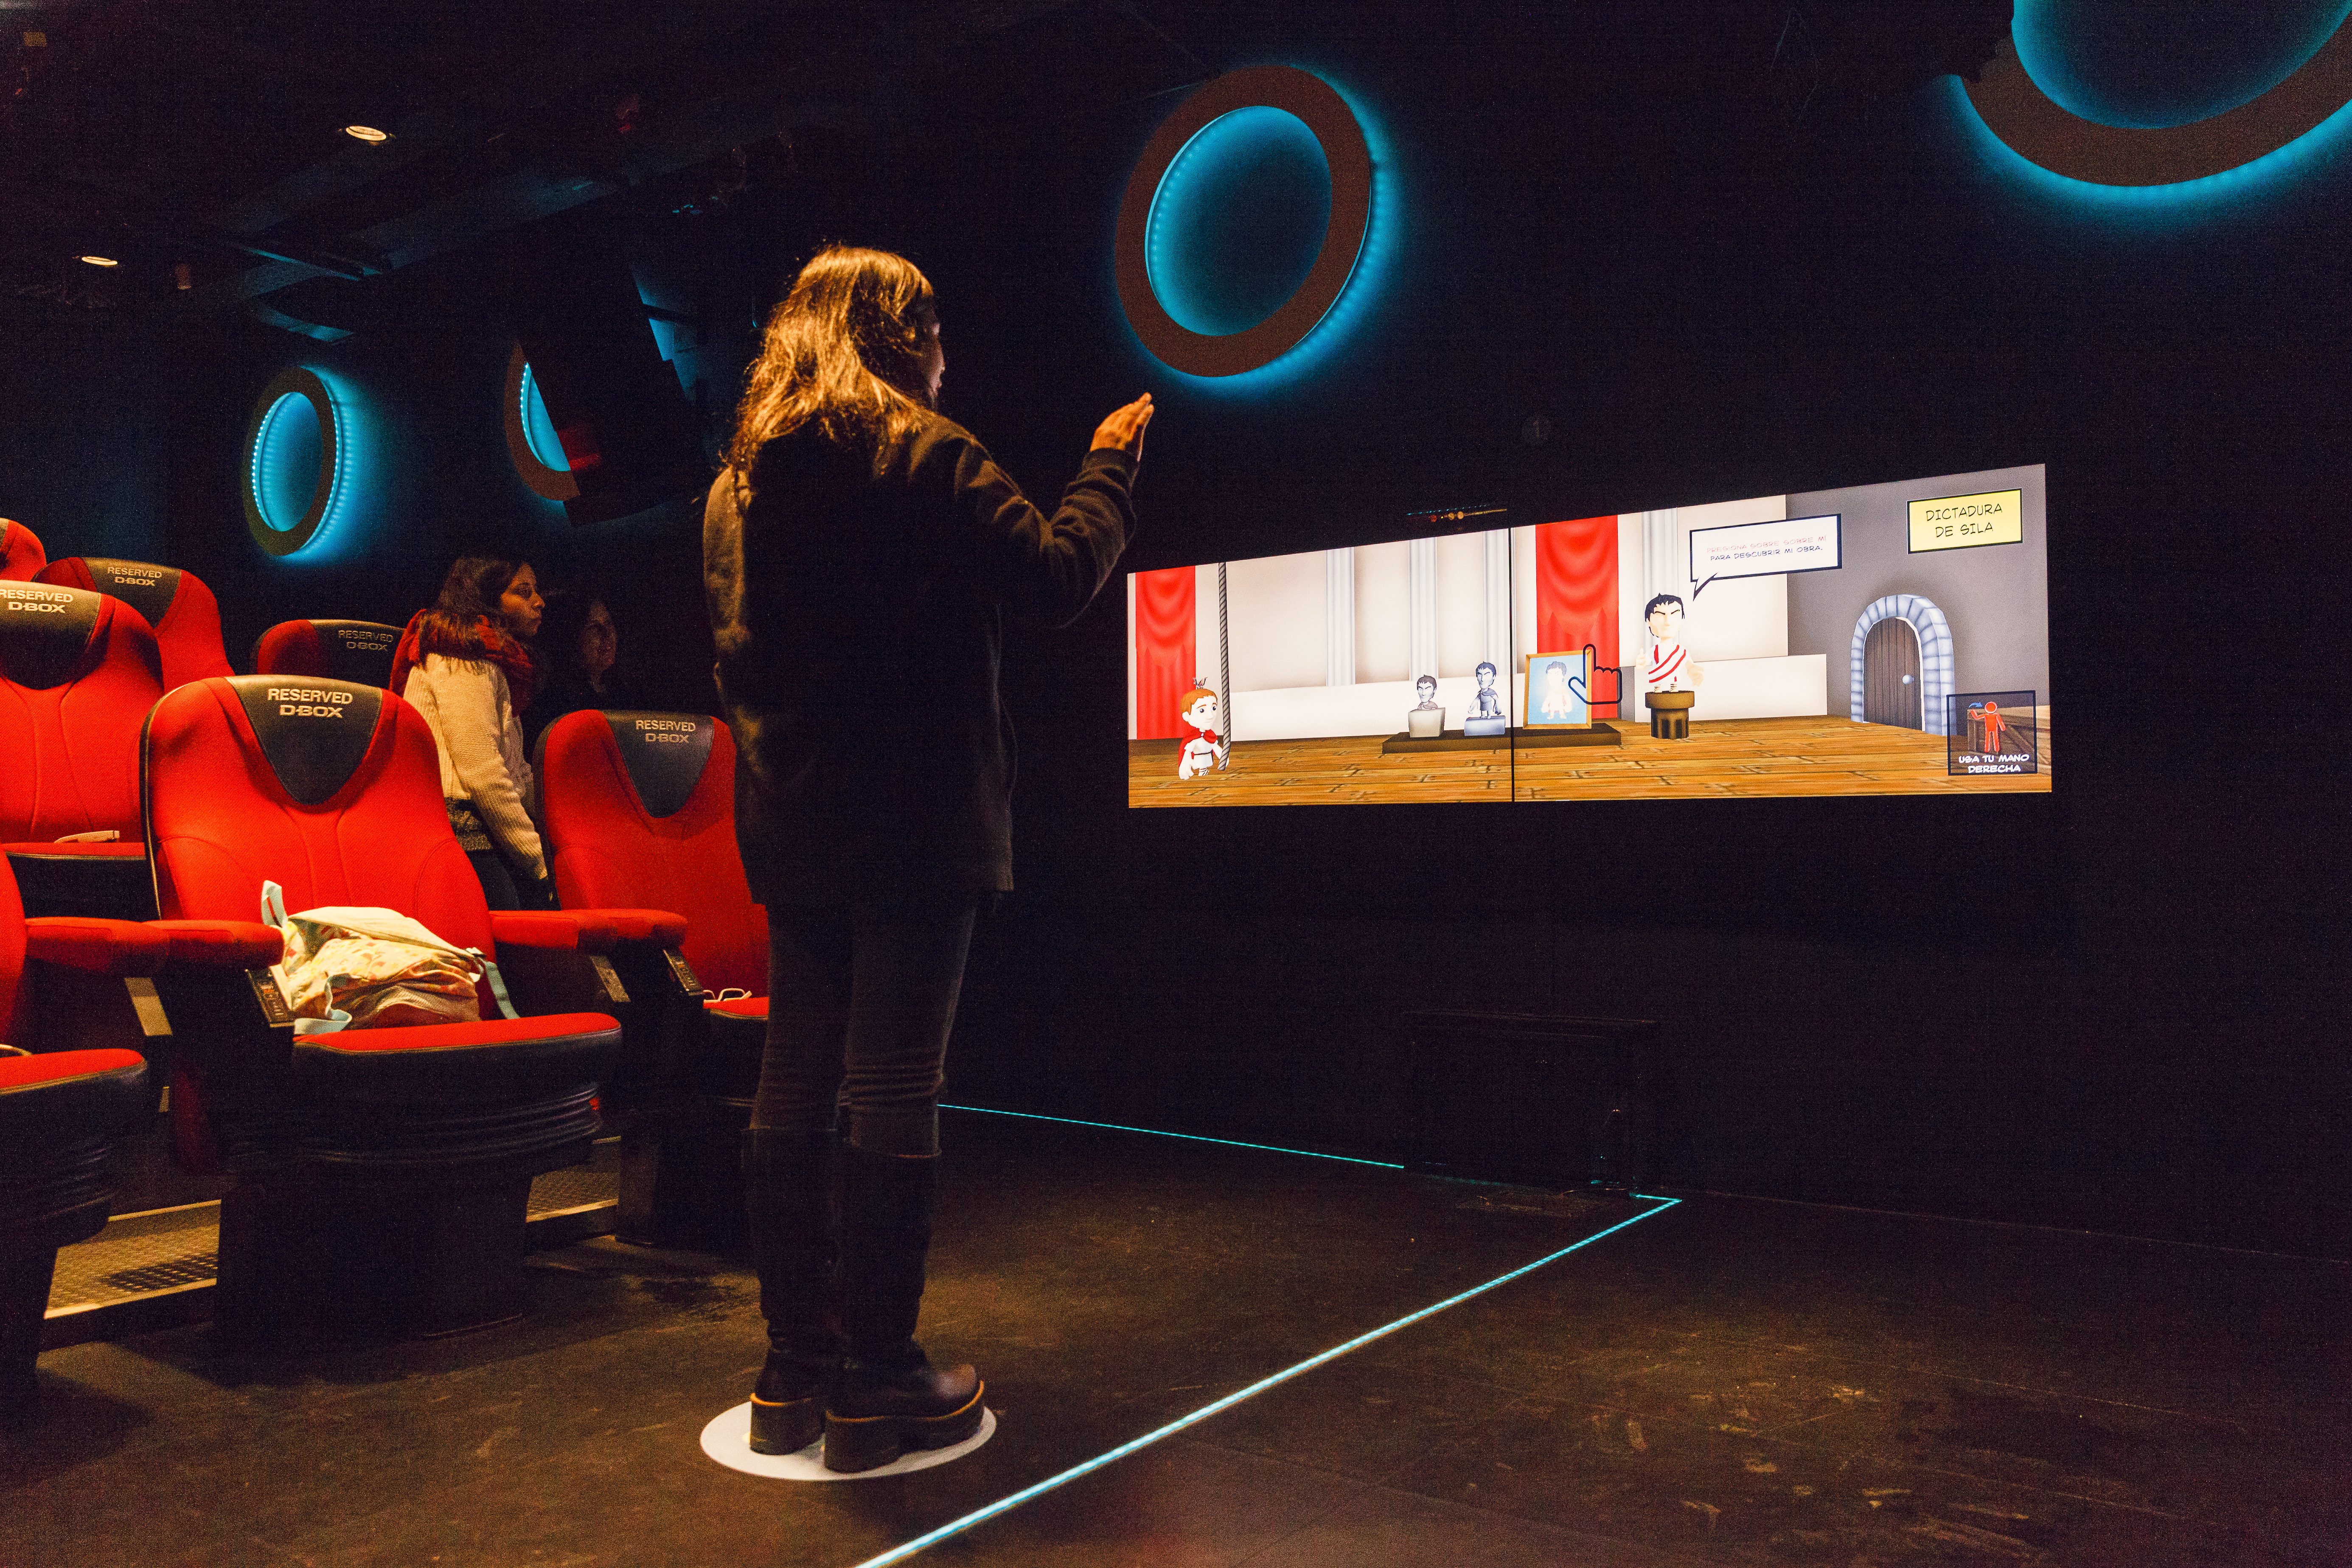
\includegraphics[scale=0.05]{musint}
\quad  
\caption{A museum interactive station}  
\label{name}  
\end{figure}
Intelligent learning environments can be used as exhibitors in museums they use embedded systems, sensors, information and communication technologies that are becoming invisible to the user as they are being integrated into physical objects, infrastructure, the environment in which we live, work and many other environments. This idea provides a good way of bridging the gap between human users and computing systems, and this motivates related research into Computing. Some of these systems use learning resources called learning objects. For the ex-change of learning objects between systems standardization initiatives have been developed and there are some implementations and repositories that manage the content using these standards. 

\section{Learning Environment}

The Learning Environment (LE) corresponds to the spaces in which the learning activities are developed, can be of three types: aulic, real and virtual. In the first it is the whole environment surrounding the student, in the context of the classroom, which focuses not only on the student, but also on the content, so the interaction with the environment will develop an interaction with the student that can be positive or negative depending the place. And has the following characteristics: 
\begin{itemize}
 \item The educator is the one who has to look for the models appropriate to their materials and the conditions of their group.
 \item They help to relate the content in an experimental and experiential way.
 \item It can be given a dynamic spatial distribution, changing as the group and the teacher consider it necessary.
\end{itemize}

The real Teaching-Learning activities are developed in the classroom, the real environment can be a laboratory, a company, clinic, library, green areas, etc. Real scenarios where you can see the application of knowledge and skills acquired, as well as the practice of attitudes and values. 

Virtual environments are those created through the use of Information and Communication Technologies, in order to provide learners with resources that facilitate their learning process, within these TICs can be cited the computer, cannon, a classroom Virtual, the use of internet where they can have access to blogs, discussion forums, chat, specialized pages where young people find fun activities, stories like solution to crosswords, puzzles, etc., that well employees contribute greatly in:
\begin{itemize}	
\item Acquisition of learning by the student.
\item Understand the nature and philosophy of distance education.
\item Identify the characteristics of students in remote locations.
\item Design and develop interactive materials that are adapted to the technology to be used, to the content, strategies and to facilitate independent study.
\end{itemize}
Learning environments are important in the day-to-day lives of people because we are in contact with them all the time in accordance with Phillips\cite{PhilMcNaKenn2010zx} a Learning Environment is a place where resources, time and reasons are available for a group of people to nurture, support and value the learning of a limited set of information. The LE are social places even when only one person is found there. 



One of the challenges facing the design of learning environments is human complexity, because each person thinks and assimilate information in different ways making it difficult to identify which resources are adequate for everyone. Intelligent learning environments (ILE) are a new type of intelligent educational system, which combines characteristics of traditional intelligent tutoring systems (ITS) \cite{john1991} and learning environments. According to Self \cite{self1998} ITS are learning systems based on computers that try to adapt to the needs of the learner. 
\begin{figure}[ht!]  
\centering  
\includegraphics[scale=1]{pizzarra}
\quad  
\caption{A kid using and intelligent chalk-board}  
\label{name}  
\end{figure}



\section{Learnign Objects.}
\section{Aim's.}
\section{Outline.}
\chapter{Art State} \label{artstate} 
In this section the state of the art in intelligent learning environments, e-learning are presented. The learning environments have been applied in
many domains
PCULS
“Personalized context-aware ubiquitous learning system for supporting effective English vocabulary learning” [Chen 2010]. This work consists of a system that supports students in English using a situational approach to learning based on the location of the learner. Detected by wireless positioning techniques, learning time, individual skills of students in English and free time, which enables students to fit your learning content to effectively support the learning of English in a school environment generating vocabulary appropriate to the situation and presenting textual information via mobile phones. When only text information shown this lack of context that was trying to capture in the vocabulary.
 

Procedure system operations:
In Step 1: The learner enters the system through the user interface where the system checks the user's account and free time available to the user.
In Step 2: After the apprentice enters the system, the student agent location automatically determines its location using a location technique based on neural networks.
In step 3 and 4: Based on the location of the learner, the context analyzer agent receives contextual information database user and context. Therefore appropriate agent finder English vocabulary seeks the context of the learner according to the analytical results of context analysis agent fits.
In step 5: Content delivery agent organizes the English learning materials discovered by the search agent material learning English as appropriate content and transmits it to the device of the learner.
In step 6: The message delivery agent transmits the learning content to the learner PDA as a web page or in the form of short message to the cell apprentice. then the trainee returns to step 2 to start the next learning cycle or exit the system, completed the learning process.
The application was tested with two sets of users. they applied a test for each user group with these results.
 
	
Display-based services through identification: An approach in a conference context.
This work combines ubiquitous computing, context, information display and [Hervas 2006] devices, to provide services to the user implicitly, with little or no user intervention feeding context information provided by sensors embedded in devices the environment. Its primary objective is to obtain service information display adaptable to changes in context, providing the same information. They base their research on the identification of users, knowing their profile, their situation in a given underlying information and much other time. Which results in a system that identifies users through RFID cards, and after analyzing generated user information service based on the information display. The whole operation of the service information display is divided into three distinct modules: Context Analysis, generation module mosaics and Composer module. The contextual model represented by an ontology proposed by the authors. The following figure shows the outline of the project is shown.
 
Every moment is available context information filtered according to the ontology and obtained from the system database and embedded sensors in the context (in principle RFID antennas and RFID tags information). The context analysis module is responsible for deciding when a change in the context must lead to changes in display devices. It is also responsible for the system database maintains the consistency of information on these changes. mosaics are generated after an analysis of the background information so that the appropriate and optimal environmental conditions to display information. The generator module provides an XML description of the Mosaic module compounder. From the description of the specific information to be displayed and the mosaic is generated is obtained, publishing through the devices of the environment and taking into account their differences.

 
Aprendizaje colaborativo basado en recursos adaptativos.

This work consists of an Adaptive Hypermedia System [Garcia, 2008], this work is focused on semi-automatic sequencing of educational resources. It builds on information that can be subjective; for example, the user's knowledge, learning style, their predilections and even evaluation; they are perceived differently depending on the context. Sequenced personalized teaching materials; using fuzzy rules and attributes to treat subjective information, involved in the learning process. I n a hypermedia system, such as the Web (W3C, 2008), users surf by  a network of resources for information or to perform some task. In the case of a student, navigation can be part of a complex learning activity; an activity may consist of: search some information, discuss the findings with other students (online), and then make a presentation where resources of different formats and sources are integrated.
In this paper propose: the architecture for a learning environment based on reusable resources, using techniques such as Adaptive Hypermedia and engine adaptation an extension to Simple Sequencing specification where a particular system of fuzzy inference. In include the use of systems fuzzy inference can facilitate the damnation of rules by the instructors, because in the learning process involved usually fuzzy variables.

\chapter{Theory and Background} \label{theoryandbg} 
This chapter overviews the background and main definitions and basic concepts, useful to the development of this investigation work.
\section{Learning environment}

	Learning environment refers to the diverse physical locations, contexts, and cultures in which students learn. Since students may learn in a wide variety of settings, such as outside-of-school locations and outdoor environments, the term is often used as a more accurate or preferred alternative to classroom, which has more limited and traditional connotations�a room with rows of desks and a chalkboard, for example.
The term also encompasses the culture of a school or class�its presiding ethos and characteristics, including how individuals interact with and treat one another�as well as the ways in which teachers may organize an educational setting to facilitate learning�e.g., by conducting classes in relevant natural ecosystems, grouping desks in specific ways, decorating the walls with learning materials, or utilizing audio, visual, and digital technologies. And because the qualities and characteristics of a learning environment are determined by a wide variety of factors, school policies, governance structures, and other features may also be considered elements of a �learning environment.�
Educators may also argue that learning environments have both a direct and indirect influence on student learning, including their engagement in what is being taught, their motivation to learn, and their sense of well-being, belonging, and personal safety. For example, learning environments filled with sunlight and stimulating educational materials would likely be considered more conducive to learning than drab spaces without windows or decoration, as would schools with fewer incidences of misbehavior, disorder, bullying, and illegal activity. How adults interact with students and how students interact with one another may also be considered aspects of a learning environment, and phrases such as �positive learning environment� or �negative learning environment� are commonly used in reference to the social and emotional dimensions of a school or class.

\section{Interactive learning environment}

	Interactive learning is a pedagogical approach that incorporates social networking and urban computing into course design and delivery. Interactive Learning has evolved out of the hyper-growth in the use of digital technology and virtual communication, particularly by students. The use of interactive technology in learning for these students is as natural as using a pencil and paper were to past generations. The Net Generation or Generation Y is the first generation to grow up in constant contact with digital media. Also known as digital natives, their techno-social, community bonds to their naturalized use of technology in every aspect of learning, to their ability to learn in new ways outside the classroom, this generation of students is pushing the boundaries of education. The use of digital media in education has led to an increase in the use of and reliance on interactive learning, which in turn has led to a revolution in the fundamental process of education.
Increasingly, students and teachers rely on each other to access sources of knowledge and share their information, expanding the general scope of the educational process to include not just instruction, but the expansion of knowledge. The role change from keeper of knowledge to facilitator of learning presents a challenge and an opportunity for educators to dramatically change the way their students learn. The boundaries between teacher and student have less meaning with interactive learning.
\section{Intelligent Tutoring System}

An intelligent tutoring system (ITS) is a computer system that aims to provide immediate and customized instruction or feedback to its learners during a task,[joseph p]without intervention from humans. ITSs have maintained the common goal of enabling learners to acquire information in a meaningful and effective manner by employing tools from a range of different technologies to direct the task at hand. There are numerous examples of ITSs being used in both education and professional settings since the mid-1920s. As a result, there is a strong relationship between ITSs, cognitive learning theories and instructional design. As with any mechanism for learning, ITSs have experienced its share of successes and limitations with continuous research investigating the best approach to addressing the dialogues and affective responses to learning.
Research in ITS organizes the "problem" in [1] knowledge about a domain, [2] knowledge about the learner, and [3] pedagogy (knowledge of teaching strategies). The major components of a typical ITS are an expert (or domain) model, student model and tutoring model. The expert model should be able to solve the problems the tutoring module submits to the students. The tutor module controls the interaction with the student, based on its teaching knowledge and comparisons between the student model and the domain knowledge. The student model reflects what the machine can infer about the student's cognitive state
\section{Intelligent learning environment}

An intelligent learning environment is a new kind of intelligent educational system, which combines the features of traditional Intelligent Tutoring Systems (ITS) and learning environments. An intelligent learning environment (ILE) includes special component to support student-driven learning, the environment module. The term environment is used to refer to that part of the system specifying or supporting the activities that the student does and the methods available to the student to do those activities [8]. Some recent ITS and ILE include also a special component called manual which provides an access to structured instructional material. The student can work with the manual via help requests or via special browsing tools exploring the instructional material on her own. An integrated ILE, which includes the environment and the manual components in addition to regular tutoring component, can support learning both procedural and declarative knowledge and provide both system-controlled and student-driven styles of learning.
\section{Fuzzy Logic}

	Zadeh introduced the term fuzzy logic in his work �fuzzy sets�, where he described the mathematics of the fuzzy set theory in 1965.
	Fuzzy logic gives the opportunity to model conditions that are defined with imprecision.
	The tolerance of the fuzzy in the process of human rezoning suggests that most of the logic behind the human rezoning is not the traditional bi-valued logic, or even the multi-valued, but the logic with fuzzy values, with fuzzy connections and fuzzy rules or inferences.

\subsection{Fuzzy sets}

	Fuzzy sets are an extension of the classic set theory and, as it name implies it, it is a set with boundaries not well defined, this means that the transition of belonging or not belonging to certain set is gradual, and this smooth transition is characterized by grades of membership that gives the fuzzy sets flexibility in modeling linguistic expressions commonly used, such as �the weather is cold� or �Gustavo is tall�.
 
Figure 2.1.Key-Value example.

\subsection{Fuzzy logic controller}

	Fuzzy control is a control method based on fuzzy logic. Just as fuzzy logic can be described simply as �computing with words rather than numbers� fuzzy control can be described simply as �control with sentences rather than equations�.
	The collection of rules is called a rule base. The rules are in the familiar if-then format, and formally the �if� side is called the antecedent and the �then� side is called the consequent.
	Fuzzy controllers are being used in various control schemes; the most used is the direct control, where the fuzzy controller is in the forward path in a feedback control system. The process output is compares with a reference, and if there is a deviation, the controller takes action according to the control strategy.
	In a feed forward control a measurable disturbance is being compensated, it requires a good model, but if a mathematical model is difficult or expensive to obtain, a fuzzy model may be useful. Fuzzy rules are also used to correct tuning parameters. If a nonlinear plant changes operating point it may be possible to change the parameters of the controller according to each operating point. His is called gain scheduling since it was originally used to change process gains. 
	A gain scheduling controller contains a linear controller whose parameters are changed as a function of the operating point in a preprogrammed way. It requires thorough knowledge of the plant, but it is often a good way to compensate for nonlinearities and parameter variations. Sensor measurements are used as scheduling variables that govern the change of the controller parameters, often by means of a table look-up.
\section{Learning object}


Learning object design raises issues of portability, and of the object's relation to a broader learning management system.
Learning objects are the basic elements of current Learning Management Systems (LMS) and are the focus of standardization initiatives whose goal is defining open technical standards and their characteristic metadata [6]. The most important initiatives are the Advanced Distributed Learning Initiative (ADL-SCORM) [7], the Instructional Management System Project (IMS) [8], the Alliance of Remote Instructional Authoring Distribution Networks of Europe (ARIADNE) [9], and the IEEE Learning Technology Standards Committee [10]. The main objective of these open standards is to enable the interoperability of learning objects between different LMSs and Learning Objects Repositories (LORS). Basic metadata schema specifications for learning objects include: Learning Object Metadata (LOM). Based on the Dublin Core metadata [11] this specification defines a set of meta- data elements that can be used to describe learning resources. LOM Includes educational, relation, technical, and classification elements [7]. Content Aggregation Model (CAM). CAM defines a package for the aggregation, distribution, management, and deployment of learning objects. Defines an organization element which contains information about one particular, passive organization of the material, the organization for now is limited to a tree structure [8]. Learner Information (LI). A collection of information about a learner or a producer of learning content, the elements are based upon accessibilities; activities; affiliations; competencies; goals; identifications; interests; qualifications, certifications and licenses; relationship; security keys; and transcripts [8]. Sequence and Navigation (SN). SN defines a method for representing the intended behavior of an authored learning experience such that any Learning Technology system (LTS) can sequence discrete learning activities in a consistent way. Provides a rule based sequencing of behaviors [7]. These standards have been the basis for various research projects in eLearning [11] and also extensions to support adaptability have been proposed [13], [14], [15]. Certain limitations of these specification initiatives have been noticed mainly regarding their weak support for the instructional design of the educational resources and pedagogy [16]. 

\section{Linda Spaces}

Linda [David Gelernter, 1985 Generative communication in Linda ACM Transactions on Programming Languages and Systems
Volume 7 , Issue 1 (January 1985), pp. 80-112] es un modelo que puede ser implementado para cualquier lenguaje que provea herramientas para crear y coordinar multiples procesos, algunas ejemplos de implementación son CppLINDA para C++, Simple C-Linda para C o PYLinda para Python. El concepto principal de LINDA es el de “Espacio de Tuplas” a través del cual los procesos se comunican. Este espacio de tuplas es una abstracción de un espacio de memoria compartida el cual se usa de manera asociativa.
El espacio de tuplas es donde se almacena la información accesible para todos los procesos. Las tuplas son colecciones de campos de algún tipo soportado por el lenguaje para el que se esta implementando. Estos campos pueden ser de dos tipos, valores de un tipo soportado o variables para recibir la información obtenida del espacio de tuplas, a las variables se les añade ? delante.
Habitualmente se definen tres operaciones sobre un espacio de
tuplas:
\begin{itemize}	
\item write(t) (out)
\begin{itemize}	
\item t es una tupla; el proceso deposita la tupla y sigue (no bloqueante)
\end{itemize}
\item take(p) (in)
\begin{itemize}
\item p es un patrón; el proceso se bloquea hasta que el espacio de tuplas le
asigna una que corresponda al patrón
\item la tupla es quitada del espacio de tuplas
\end{itemize}
\item read(p) (rd)
\begin{itemize}
\item versión del “take” en que la tupla que le es asignada no se elimina del
espacio de tuplas
\item puede haber varios read simultáneos
\end{itemize}
\end{itemize}
\begin{figure}[ht!]  
\centering  
\includegraphics[scale=1]{linda}
\quad  
\caption{E-Learning}  
\label{keyvalue}  
\end{figure}

En el modelo básico las tuplas son bastante simples. Aqui se muestra una definicion general 
Let A be a set of typed elements, called atoms, for which a mapping.
 
\begin{equation}
EQ_{A} : A \times A \to \{ 0, 1 \} 
\end{equation}

%is assumed to be defined. The set of tuples TA is defined as follows: 
\begin{enumerate}	
\item for any a \( \in \) A, [a] belongs to \( \tau_{A} \)
%\item for any \[a\] \boldsymbol{\tau}_{A}, \[\[la\]\] belongs to \boldsymbol{\tau}_{A} 
%\item if [el] and [e2] belong to \boldsymbol{\tau}_{A}, then [e1 e2] also belongs to \boldsymbol{\tau}_{A}  
\end{enumerate}



\section{NoSQL}

In computing, NoSQL (sometimes called "not only SQL") is a broad class of systems management databases that differ from the classical model of relational database management system (RDBMS) in important aspects, the most prominent is that they are not using SQL as the primary query language. The stored data do not require fixed structures such as tables, typically do not support JOIN operations, not fully guarantee ACID (atomicity, consistency, isolation and durability), and usually scale well horizontally. The NoSQL systems are sometimes called "not only SQL" to underline the fact that they can also support query languages like SQL. The NoSQL databases Systems grew with major Internet companies like Google, Amazon, Twitter and Facebook. These had to face challenges with data processing than traditional RDBMS not solved. With the growth of the web in real time there was a need to provide processed information from large volumes of data that had more or less similar horizontal structures. These companies realized that the performance and real-time properties were more important than consistency, in which the traditional relational data bases devoted a lot of processing time. 
In that sense, often, NoSQL databases are highly optimized for operations retrieve and add, and usually do not offer much more than the functionality of store records (eg key-value storage) that we can see on figure \ref{keyvalue}. The loss of flexibility at run time compared to conventional systems SQL, is offset by significant gains in scalability and performance when it comes to certain data models.

 \begin{figure}[ht!]  
\centering  
\includegraphics[scale=1]{nosqlejemplo}
\quad  
\caption{Key-Value Storage}  
\label{keyvalue}  
\end{figure}

\subsection{Key-Value example}

Typically the modern relational data bases have shown little efficiency in certain applications that use data intensively, including indexing of a large number of documents, presentation pages sites with high traffic, and sites audiovisual streaming. Typical implementations of RDBMS have tuned either for a small but frequent reads and writes or a large set of transactions that have few write accesses amount. On the other hand it can serve NoSQL lot of load of reads and writes.
\subsection{Advantages of NoSQL systems}

This way of storing information provides certain advantages over relational models. Between the most significant advantages can include:
They are executed in machines with limited resources: These systems, unlike based systems SQL, not just require computer, so they can be mounted on machines of a lower cost.
Horizontal Scalability: To improve the performance of these systems is achieved simply adding more nodes, with the only operation of the system indicate which nodes are available.
Can handle large amounts of data: This is because it uses a distributed structure, Hash many cases using tables.
Do not generate bottlenecks: The main problem with SQL systems is that they need to transcribe each sentence to be executed, and each complex sentence also requires a level even more complex implementation, which is an entry point in common, that before many requests can slow down the system.

\subsection{Main differences with SQL databases}

Some of the most remarkable differences we can find between NoSQL systems and SQL systems are:
Do not use SQL as a query language. Most NoSQL databases avoid using this kind of language or use it as a language support. To give some examples, Cassandra uses CQL language, MongoDB uses JSON or BigTable uses GQL.
Not use fixed structures as tables for storing data. Let you use other types of storage models as key-value systems, objects or graphs.
Tend not allow JOIN operations. By having a data volume so extremely large is often desirable to avoid the JOIN. This is because, when the operation is not the search for a key, the overhead can become very costly. The most straightforward solutions consist of denormalising data or perform the JOIN by software in the layer application.
Distributed architecture. The relational databases are typically centralized in a single machine or in a master-slave structure, however in cases NoSQL information it can be shared across multiple machines through mechanisms of distributed hash tables.

\subsection{Types of NoSQL databases}

Depending on how you store the information, we can find various types other than NoSQL databases. Consider the most commonly used types.
Key-Value Database: They are the base model popular NoSQL data, besides being the simplest in terms of functionality. In this type of system, each element is identified by a unique key, allowing the retrieval of information very quickly, which is usually stored information as a binary large object (BLOB). They are characterized by being very efficient for both readings and for scriptures. Examples of this type are Cassandra, HBase or BigTable.
 


Document databases: They are the base model popular NoSQL data, besides being the simplest in terms of functionality. In this type of system, each element is identified by a unique key, allowing the retrieval of information very quickly, which is usually stored information as a binary large object (BLOB). They are characterized by being very efficient for both readings and for scriptures we can see an example of this kind of data base on the figure 2.3. Examples of this type are Cassandra, HBase or BigTable. 
\begin{figure}[ht!]  
\centering  
\includegraphics[scale=1]{basededatosdoc}
\quad  
\caption{Document Database Example}  
\label{bddd}  
\end{figure}

Graph databases: In this type of databases, information is represented as nodes of a graph and its relations with the edges thereof (Figure 2.4), so that you can make use of graph theory to cover it. To remove the most of this type of database, its structure must be fully normalized, of so that each table has a single column and each relationship both. This type of database provides a more efficient navigation between relationships vs a relational model. Examples of this type are Neo4j, InfoGrid or Virtuoso.

\begin{figure}[ht!]  
\centering  
\includegraphics[scale=0.75]{Graph-database}
\quad  
\caption{Graph Database Example}  
\label{bdg}  
\end{figure}

\subsection{Examples of NoSQL databases}

Here are some examples of the most commonly used nosql databases.

Cassandra: This is a database created by Apache key-value type. It has its own language for CQL (Cassandra Query Language) queries. Cassandra is a Java application so it can run on any platform that has the Java Virtual Machine.
 
\begin{figure}[ht!]  
\centering  
\includegraphics[scale=0.1]{cassandra}
\quad  
\caption{Nosql Database Cassandra}  
\label{bdg}  
\end{figure}


MongoDB: This is a database created by 10gen document-oriented type, Free scheme is meaning that each input can have a different data schema that has nothing to do with the rest stored records. It's pretty quick to run its operations as it is written in C ++ language. For information storage, uses a proprietary system known document with the BSON name, which is an evolution of the popular JSON but with the peculiarity that can store binary data. Soon, MongoDB has become one of the bases of popular NoSQL data by developers.
 
\begin{figure}[ht!]  
\centering  
\includegraphics[scale=1]{mongo}
\quad  
\caption{Nosql Database MongoDB}  
\label{bdg}  
\end{figure}


CouchDB: It is a system created by Apache and written in Erlang language that works in most POSIX systems, including GNU / Linux and OSX, but not in Windows systems. The most important features include the use of Restfull HTTP API as an interface and JavaScript as the main language of interaction. For storage of data files used JSON.Allows creation of views, which are the mechanism that allows the combination of documents return values of several documents, ie, CouchDB allows performing operations JOIN Typical SQL.

\begin{figure}[ht!]  
\centering  
\includegraphics[scale=1]{couchdb}
\quad  
\caption{Nosql Database CouchDB}  
\label{bdg}  
\end{figure}


\chapter{The Proposed Method} \label{proposmeth} 
The proposed method is based in a previous architecture presented in [46] used in an e-learning platform (Protoboard) where the context involves characteristics referring
the student environment as well as their performance in previous learning activities.
In this chapter, an architecture for developing interactive learning environments is proposed. The architecture allows the use of techniques of adaptive hypermedia systems and use in interactive environments. This architecture has as resources environmental learning objects, which are presented to users through the various devices that can be part of this environment and are organized by a sequence based on Simple Sequencing. Also a new method to automate the measurement of the level of attention of the user without using invasive methods. In Figure \ref{arquitectura} we can observe the components of this architecture. As this environment has multiple configurations of use, sometimes it can help a fuzzy inference system to adapt the information presented by the environment to users. The components of the architecture are described in detail in this chapter.

\begin{figure}[ht!]  
\centering  
\includegraphics[scale=1]{arquitectura}
\quad  
\caption{Adaptive Learning Environment Architecture}  
\label{architecture}  
\end{figure}


\section{Environment}
%Los ambientes inteligentes son espacios con sistemas embebidos, sensores y tecnolog�as de informaci�n y comunicaci�n que se van haciendo imperceptibles para el usuario a media que van siendo integrados en objetos f�sicos, infraestructuras, el entorno en que vivimos, el trabajo y muchos otros ambientes. Los ambientes inteligentes interactivos facilitan herramientas con las cuales los usuarios pueden interactuar, lo que hace que este espacio sea interactivo por lo que la computaci�n se aproxima m�s al usuario. Existen otros tipos de ambientes como e-learning que son ambientes de aprendizaje virtuales donde un usuario aprende individualmente ciertos temas a partir de objetos de aprendizaje. Los trabajos en este tipo de ambientes de aprendizaje han utilizado diferentes t�cnicas para secuenciar y seleccionar los objetos de aprendizaje para cubrir las necesidades de aprendizaje del individuo como el secuenciado simple (referencia a la tesis del profe). 

Intelligent environments are spaces with embedded systems, sensors and information and communication technologies that are becoming imperceptible to the average user that are being integrated into physical objects, infrastructures, the environment in which we live, work and many other environments.
Intelligent interactive environments provide tools with which users can interact, which makes this space interactive so that the computer is closer to the user. There are other types of environments such as e-learning that are virtual learning environments where a user learns individually certain topics from learning objects. The work in this type of learning environments has used different techniques to sequence and select learning objects to cover the learning needs of the individual such as simple sequencing (referencia a la tesis del profe). 

\begin{figure}[ht!]  
\centering  
\includegraphics[scale=1]{elearning}
\quad  
\caption{E-Learning}  
\label{keyvalue}  
\end{figure}
The problem we notice is that most of them focus on a single solution, either oriented to learning, modify the environment, that handle only one user at a time. In reviewing the literature we realized that by combining certain standards there is an improvement in the user's learning experience. Currently there are certain limitations with intelligent environments such as:
\begin{itemize}	
\item Learning environments are designed so that learning objects are used by one user at a time.
\item Contextual information is sometimes not considered.
\item Usually the environment can not be taken to other places without having to make modifications.
\item Some works with environments use devices that are not as advanced as they are now, and have become more accessible economically.
\end{itemize}

%Proponemos generar un ambiente que gracias a un servicio web sea capaz de atacar todas las limitaciones que observamos en los ambientes de aprendizaje actuales. Gracias a los servicios web podemos crear repositorios que pueden estar disponibles siempre y cuando exista una conexion a internet, pero que pasa con aquellos lugares donde no exista tal conexion, para estos casos se puede llevar un repositorio que sirva como local para poder obtener los objetos de aprendizaje o el contenido. Ademas el ambiente esta centrado para atender a un grupo de usuarios.
We propose to generate an environment that thanks to a web service is capable of attacking all the limitations that we observe in the current learning environments. Thanks to the web services we can create repositories that can be available as long as there is an internet connection. But what about those places where there is no such connection? For these cases you can take a repository that serves as a local to be able to obtain learning objects or content. In addition the environment is focused to serve a group of users.

%El ambiente de aprendizaje propuesto tiene proyectados varios usos, el primero de ellos y obviamente como ambiente de aprendizaje, como exhibidor de museo, entrenamiento, entretenimiento, publicidad, juegos. y esto es posible gracias al servicio web que permite utilizar diferentes objetos de aprendizaje y de diferentes tipos en cualquier dispositivo sea capaz de correr un navegador web y que este disponible.
The proposed learning environment has several uses, the first of them and obviously as a learning environment, as a museum exhibitor, training, entertainment, advertising, games. And this is possible thanks to the web service that allows to use different learning objects and of different types in any device that is able to run a web browser and that it is available.
Then we will be concerned with the learning part, the modification of the environment and the user resulting in a learning environment that can be manipulated or adjusted to the needs of the users. In order to carry out this, we propose a new learning object methodology, which we will call "Environmental Learning Object", this object will be used in a learning environment where users can interact with it. We will speak more specifically about this proposal later.

\section{Proposed learning object}
Ya hablamos en capitulos anteriores sobre los objetos de aprendizaje y sobre su importancia para este proyecto en esta seccion hablaremos sobre el nuevo tipo de objeto de aprendizaje que estamos proponiendo, la definicion de 
standard learning object is defined in \cite{wayneh}. 
en los ambientes de aprendizaje The teacher prepares teaching materials using content from various sources; select different pieces of information that subsequently assembled to form the course or class to teach. Learning objects are based on this methodology, seeing the didactic content as a component that is designed to combine with others and to be used in different contexts; learning objects usually have the following characteristics: 
�	They are self-contained. Each learning object can be used independently. 
�	Are reusable. A learning object can be used in different contexts, for multiple purposes. 
�	Can be added. Learning objects can be grouped into collections, after being presented with a traditional course structure. 
�	Are labeled with metadata. Each learning object has associated certain in-formation that describes it. This facilitates reuse by automatic means.
Entonces nuestra tarea es desarrollar un metodo que le permita al maestro seleccionar piezas de informacion que sean contextualmente relevantes para el usuario.
\subsection{Linda Spaces}
Para distribuir los onjetos de aprendizaje sobre los dispositivos disponibles tomamos como referencia el lenguaje de coordinacion Linda Spaces.
Linda [David Gelernter, 1985 Generative communication in Linda ACM Transactions on Programming Languages and Systems
Volume 7 , Issue 1 (January 1985), pp. 80-112] es un modelo que puede ser implementado para cualquier lenguaje que provea herramientas para crear y coordinar multiples procesos, algunas ejemplos de implementaci�n son CppLINDA para C++, Simple C-Linda para C o PYLinda para Python. El concepto principal de LINDA es el de �Espacio de Tuplas� a trav�s del cual los procesos se comunican. Este espacio de tuplas es una abstracci�n de un espacio de memoria compartida el cual se usa de manera asociativa.
El espacio de tuplas es donde se almacena la informaci�n accesible para todos los procesos. Las tuplas son colecciones de campos de alg�n tipo soportado por el lenguaje para el que se esta implementando. Estos campos pueden ser de dos tipos, valores de un tipo soportado o variables para recibir la informaci�n obtenida del espacio de tuplas, a las variables se les a�ade ? delante.
Habitualmente se definen tres operaciones sobre un espacio de
tuplas:
\begin{itemize}	
\item write(t) (out)
\begin{itemize}	
\item t es una tupla; el proceso deposita la tupla y sigue (no bloqueante)
\end{itemize}
\item take(p) (in)
\begin{itemize}
\item p es un patr�n; el proceso se bloquea hasta que el espacio de tuplas le
asigna una que corresponda al patr�n
\item la tupla es quitada del espacio de tuplas
\end{itemize}
\item read(p) (rd)
\begin{itemize}
\item versi�n del �take� en que la tupla que le es asignada no se elimina del
espacio de tuplas
\item puede haber varios read simult�neos
\end{itemize}
\end{itemize}
\begin{figure}[ht!]  
\centering  
\includegraphics[scale=1]{linda}
\quad  
\caption{E-Learning}  
\label{keyvalue}  
\end{figure}

En el modelo b�sico las tuplas son bastante simples Aqui se muestra una definicion general 


\subsection{ELO}
We propose a learning environment that uses a new type of learning object which we call "Environmental Learning Object" (ELO) these objects include additional metadata that can be used to identify and manage content for their use in ubiquitous devices: we considered input and output devices e.g. interactive table's, wall projections, monitors, tablets, cameras, microphones and speakers.
By tagging through the metadata we can make a selection of learning objects to create and manage different contexts when applied to a learning environment.

Where each learning object is selected and routed to a device that operates its utility like a sound file that can�t be used on a monitor maybe on a Smartphone or a tablet pc, these are the types of problems that can occur when using these learning objects. Also this ELO will give contextual information for feedback. 

\subsection{Formal definition.}
Objeto de Aprendizaje Ambiental (OAA) es un objeto de aprendizaje que permite la distribuci�n de contenido a diversos dispositivos con la condici�n de que deben estar disponibles y ser compatibles en un ambiente de aprendizaje interactivo.
Un objeto de aprendizaje ambiental (OAA) se determina por la tupla <O,D> donde O es un conjunto de objetos de aprendizaje y D es un conjunto de Dispositivos.
OOA=((O,D),D)

Donde un objeto de aprendizaje o ? O objetos de aprendizaje como entidades, digitales o no digitales, que pueden ser utilizadas para promover el aprendizaje, educaci�n o entrenamiento.
Y un dispositivo d ? D dispositivos con la condici�n de que deben estar disponibles y ser compatibles en un ambiente de aprendizaje interactivo.

\subsection{Formal definition.}
\section{Fuzzy simple sequencing}
Simple sequencing standard[18] [19], which allows sequencing of this type of learning objects. First an activity tree with n number of activities is determined by the teacher, selecting the learning objects to be used per activity and adding fuzzy pre-condition rules that consider the context and user model to determine the sequence, for example:
IF Context.Temperature is HIGH and Session.Activity.Place is OUTSIDE
THEN
this.Precondition. = SKIP.
Then context information is obtained from users using the sensors mentioned above, each activity will have 1 or more environmental learning objects, thanks to the metadata included in the learning objects will be displayed in the appropriate device for example if we have a web page can be displayed on a monitor, a questionnaire on a tablet, a video projected on a wall, sound on speakers, an interactive game on the table as we can see in Figure 3.
The main components of the Simple Sequencing standard are the Learning Activities and the Activity Tree. A Learning Activity is defined as a pedagogically neutral unit of instruction, knowledge, evaluation, etc. Learning Activities can have nested sub-activities arbitrary depth. 
There is an implicit hierarchy of containers in the tree. Depending on the application concept labels can be applied to learning activities. Only leaf nodes can be associated with Resources Activity (the equivalent of Learning Objects).An example of the configuration obtained by sequencing can be observed in Figure 3.2. The tree is traversed as follows from the root there is the General activity (can be any subject in particular) with 2 nodes in it, we see that has the attribute "forwardOnly" on true, this means they have to be traveled sequentially by users, the first activity is a pre-evaluation, which is associated with a learning object in this case a test that contains a rule that makes the activity is carried out or otherwise will not advance to the next activity, as specified in the Pre\_condition rule.
When a learning sequence is generated learning activities are established and they not change, what changes is the action as if you skip, performed, jump, hide, repeat or show an activity, this decision is taken by the rules of precondition. In this paper we seek to generate diversity of resources displayed in the activities adapting the resources of the activity to the user,  for example we have an introductory activity of a particular subject and 2 users of different ages perform the activity, the first user of 25 years will be shown more detailed and textual information, while the second user of 6 years of age is in a very early stage of learning resources that show you are easier to understand and have more audio-visual con-tent. With fuzzy logic generate inputs for use in the precondition rules for example: fuzzy rule if user.age is low and user.academic\_level is low then user.level is begginer. On the precondition rule we will use the output of the fuzzy rule will use the output of that fuzzy rule as follows if user=begginer then pre\_condition = show. Thus a set of resources is obtained for a novice user and these are shown on the right devices for each resource through a web browser running in this device as we can see on the figure 1.

\section{Devices}
\section{Master / User}
\section{Engagement}
The other way to obtain user information was by Kinect Sensor and is a bit more complex because the sensor provides enough information the sensor detects a user can give: 
� engage 
� looking away 
� happy 
� left eye closed 
� right eye closed
� mouth open 
� mouth moved 
� wearing glasses 
� yaw pitch and roll of the face
Each of these data the sensor assigned one of the following Yes, No, Maybe and Unknown values; unknown data were discarded since in the sensor documentation was saying that this data could be�not sensing� and therefore not considered valid data. Only in the face position was a numerical data, the sensor generated an average of 14 records per second of these values sometimes less for a short time when the sensor lost sight of the user but was usually between 1 to 10 seconds.
Full activity was carried out in 4 minutes 10 seconds so if the sensor not loses sight of the user throughout the activity it generates about 3500 records. From the above list of data we decided to use only engage, looking away happy and others are captured but used as they are not relevant to what we are measuring. To get textual results perform a normalization by a count of each event every 10 seconds since the data generated by the sensor are textual normalized by assigning numbers to strings for example Yes = 2, Maybe = 1 and No = 0 then for every 10 seconds of activity the Yes, No and Maybe was counted.
As the activity lasted 4:10 we decided to count the sensor event every 10 seconds, at the end we gained an average of 140 records for each period of 10 seconds. Here I was a problem, as the number of records varied by user we had to think about how to normalize this data, as records were recorded and distributed yes, maybe, no the solution was to take a percentage of each of the records obtained by which thus we could handle and sensor data.
\chapter{Experiments and Results} \label{expres} 
\section{Experiments}
This study is divided into 2 experiments, the first part was conducted with visitors to the museum’s spin Tijuana where 21 users divided into 2 groups participated, the first has 10 users between 6 and 11 years 50% men and 50% women and the second group consisted of 11 users 11 and older 66 % men 44 % women. In the second part of the study 41 users of the Technological Institute of Tijuana were used aged between 18 and 50 years 66 % men 34 % women. 
For this study is required to show images, videos and somehow observe the user, that is why many devices that met these needs as a computer to server, 2 laptops, one 7-inch tablet, headphones, 3 projectors, 2 monitors, cameras, sensors (Kinect 2.0) etc. were used. 
In the first part of the study users immersed in an exhibitor that gave them visual and aural information as shown in Figure 1 on a topic selected based on various criteria, such as the location of the study on this occasion was a interactive museum and the festival of children’s day approaching we try to use a simple theme and it will bring awareness so we decided to use the theme of water where information was displayed as the uses of the same, its cycle, forms of energy that could generate, health, and the importance of it for the planet. Each of users are generating an account on the system to register their activity, after that we were made a brief explanation of how it worked the exhibitor others based on observation no longer required this explanation. The user took a tablet that was the how the user interacted with the exhibitor, with which had control of the flow of information, as the information was a sequence at the end of the last activity was a questionnaire on the information received besides a survey.
The second part of the study was very similar to the first one that had some small modifications and additions, now the user no longer had control flow only observe and also to observe the user now will take video and sensor, the theme of the exhibition were video games and film as the age of the users would go for almost 17 years and older could be topics of their interest. In the same way as in the first part each user had an account to record the activity only this occasion the data produced by the sensor and videos captured by the camera would be recorded, and in the same way as in the first part at the end we surveyed the users.
For the first part of the study we get data from the survey conducted at the end, in the second they are collected and used data from sensors, this data were a bit more complex, first we need an observer to evaluate the user manually, where the observer determined whether the user was putting attention to what he saw or distracted and based on that assigned a level of attention on a scale of 1 to 3 where 1 is little attention 2 average attention and 3 very attentive. 
The other way to obtain user information was by Kinect Sensor and is a bit more complex because the sensor provides enough information the sensor detects a user can give: 
• engage 
• looking away 
• happy 
• left eye closed 
• right eye closed
• mouth open 
• mouth moved 
• wearing glasses 
• yaw pitch and roll of the face
Each of these data the sensor assigned one of the following Yes, No, Maybe and Unknown values; unknown data were discarded since in the sensor documentation was saying that this data could be”not sensing” and therefore not considered valid data. Only in the face position was a numerical data, the sensor generated an average of 14 records per second of these values sometimes less for a short time when the sensor lost sight of the user but was usually between 1 to 10 seconds.
Full activity was carried out in 4 minutes 10 seconds so if the sensor not loses sight of the user throughout the activity it generates about 3500 records. From the above list of data we decided to use only engage, looking away happy and others are captured but used as they are not relevant to what we are measuring. To get textual results perform a normalization by a count of each event every 10 seconds since the data generated by the sensor are textual normalized by assigning numbers to strings for example Yes = 2, Maybe = 1 and No = 0 then for every 10 seconds of activity the Yes, No and Maybe was counted.
As the activity lasted 4:10 we decided to count the sensor event every 10 seconds, at the end we gained an average of 140 records for each period of 10 seconds. Here I was a problem, as the number of records varied by user we had to think about how to normalize this data, as records were recorded and distributed yes, maybe, no the solution was to take a percentage of each of the records obtained by which thus we could handle and sensor data.
\section{Results}
\chapter{Environment Evaluation} \label{enveva} 
\chapter{Conclutions} \label{conclu} 
En este trabajo de investigaci�n, se desarrollo un ambiente de aprendizaje interactivo con m�ltiples usos como exhibidor de museo, entretenimiento, publicidad, etc. La principal caracter�stica de este ambiente de aprendizaje es que cuenta con un objeto de aprendizaje especial que al combinarse con el ambiente le permite ser lo que se mencionaba antes.
El desempe�o de este ambiente lo medimos en varias pruebas con usuarios reales, el ambiente en sus primeras versiones fue probado con usuarios �locales� (Usuarios al alcance del laboratorio) para medir la aceptaci�n de este tipo de tecnolog�a y que tan f�cil era de utilizar el ambiente en la cual tuvimos buenos resultados. 
En la segunda versi�n nos trasladamos al museo interactivo de Tijuana El trompo donde el objetivo de la prueba fue usarlo con usuarios de diversas edades y observar las reacciones de estos mismos desde esta versi�n utilizamos el sensor de Kinect 2 para observar el usuario pero la informaci�n obtenida no fue lo suficientemente buena para utilizarla, en esta ocasi�n el ambiente con informaci�n dada por el usuario era capaz de modificar la informaci�n mostrada en un intento por adaptar la informaci�n y ser m�s atractiva para el usuario. Al no poder utilizar la informaci�n dada por el sensor optamos por conservar las encuestas que les aplicamos a los usuarios las cuales mostraron muy buena aceptaci�n en su mayor�a, los pocos que no estuvieron de acuerdo fueron ni�os menores de 6 a�os los cuales mostraron poco inter�s y un nivel de distracci�n un poco alto esto lo atribuimos a que los ni�os eran extranjeros y no dominaban muy poco idioma espa�ol que era el idioma que manejaba el ambiente.   
En la �ltima versi�n del ambiente fue utilizado en el instituto tecnol�gico de Tijuana utilizando un grupo de usuarios m�s homog�neo los cuales eran alumnos y algunos maestros de la escuela, en esta prueba los usuarios adem�s de ser observados por el sensor tambi�n se les tomo video para analizarlo y tener una referencia para los resultados de la clasificaci�n de datos dada por el sensor adem�s se le aplico una encuesta a los usuarios para identificar los gustos en cuanto a informaci�n y los dispositivos que utilizan los usuarios. cada una de las pruebas el ambiente evolucionaba gracias a la informaci�n proporcionada por los usuarios de ir de algo muy simple como solo mostrar im�genes a mostrar videos, reproducir audios. Luego de ciertas modificaciones pudimos manipular contenido y secuenciarlo.


\appendix
%% Cap'itulos incluidos despues del comando \appendix aparecen como ap'endices
%% de la tesis.
\chapter{Technical support of installation}\label{appendixa}
%\begin{singlespace}
\textbf{\large{Dependencies of the application}}
\begin{itemize}
\item Django framework 1.3-1.7.\\ Url: 
\url{https://www.djangoproject.com/download/}
\item Redis. \\
Url: \url{https://redis.io/}
\item CouchDB. \\
Url: \url{http://couchdb.apache.org/}
\item SQlite \\
Url: \url{https://www.sqlite.org/}
\item Visual Studio 2015. \\
Url: \url{https://www.visualstudio.com/downloads/}
\item PostgreSQL database. 
\\Url: \url{http://www.postgresql.org/}
\item Psycopg2 connection to database. \\
Url: \url{http://initd.org/psycopg/docs/install.html}
\item Kinect for Windows SDK 
Url:\url{https://www.microsoft.com/en-us/download/details.aspx?id=44561}
\end{itemize}
%\end{singlespace}
%\include{apendiceB}
%\include{apendiceC}

\bibliography{biblio}
%% Incluir la bibliograf'ia. Mirar el archivo "biblio.bib" para m'as detales
%% y un ejemplo.


\end{document}
